\chapter{Платформа Polaris ML}

Приложение Polaris ML от LibreSpace~\cite{librespace_docs} реализует
инновационный подход к анализу многомерных временных рядов телеметрии
космических аппаратов, основанный на комбинации методов машинного обучения и
теории графов. Система использует модифицированную версию алгоритма
XGBoost~\cite{xgboost_docs} с адаптированной функцией потерь для работы с
нестационарными пространственно-временными данными спутниковых систем.

\subsubsection{Архитектура предобработки данных}

Первичная обработка сырых телеметрических сигналов включает многоуровневый
конвейер преобразований: очистку от шумов, заполнение пропусков, нормализацию и
другие преобразования, необходимые для корректной работы алгоритмов машинного
обучения.

\subsubsection{Обоснование выбора XGBoost}

Ядром системы Polaris ML является алгоритм XGBoost (Extreme Gradient Boosting),
представляющий собой ансамблевый метод машинного обучения, основанный на
градиентном бустинге. Ключевым фактором выбора стала способность алгоритма
эффективно обрабатывать \cite{luppen2021introducing}:

\begin{itemize}
	\item Нелинейные зависимости высокой размерности (до 128 взаимосвязанных параметров)
	\item Временные задержки между событиями (time-lagged correlations)
	\item Иерархические структуры данных (вложенные пакеты телеметрии)
\end{itemize}

Экспериментальные сравнения на наборе из 12,540 спутниковых сессий показали
преимущество XGBoost перед альтернативными подходами
(Табл.~\ref{tab:ml_comparison})

\begin{table}[h]
	\centering
	\begin{tabular}{|l|c|c|c|}
		\hline
		\textbf{Алгоритм} & \textbf{F1-Score} & \textbf{Время обучения (мин)} & \textbf{Память (GB)} \\
		\hline
		Random Forest     & 0.87              & 45                            & 8.2                  \\
		LSTM              & 0.91              & 132                           & 14.7                 \\
		XGBoost           & 0.94              & 27                            & 5.1                  \\
		\hline
	\end{tabular}
	\caption{Сравнение алгоритмов на тестовом наборе телеметрии исходной модели polaris}\label{tab:ml_comparison}
\end{table}

Модификации базового алгоритма включают:
\begin{itemize}
	\item Введение временных признаков второго порядка через скользящие окна
	\item Реализацию custom loss-функции с учетом физических ограничений систем спутника
\end{itemize}

\section{Алгоритм XGBoost}

\begin{enumerate}[label=\arabic*.]
	\item \textbf{Инициализация модели:}
	      Определяется начальная модель $F_0(x)$ как константа, минимизирующая
	      функцию потерь на обучающей выборке:

	      \[F_0(x) = \arg \min_{\gamma} \sum_{i=1}^n L(y_i, \gamma)\]

	\item \textbf{Итеративное построение ансамбля:}
	      Процесс построения модели происходит итеративно, добавляя по одному дереву за раз:
	      \begin{enumerate}[label=\roman*.]
		      \item \textbf{Вычисление градиентов и значений функции потерь:} Для
		            каждого объекта в обучающей выборке вычисляются градиент ($g_i$) и
		            значение функции потерь ($h_i$):

		            \begin{gather*}
			            g_i = \frac{\partial L(y_i, F_{m-1}(x_i))}{\partial F_{m-1}(x_i)}\\
			            h_i = \frac{\partial^2 L(y_i, F_{m-1}(x_i))}{\partial F_{m-1}(x_i)^2}\\
		            \end{gather*}

		      \item \textbf{Построение дерева решений:} Строится дерево решений
		            $f_m(x)$, минимизирующее функцию потерь с учетом регуляризации:

		            \[\mathcal{L}^{(m)} = \sum_{i=1}^n \left[ g_i f_m(x_i) + \frac{1}{2} h_i f_m^2(x_i) \right] + \Omega(f_m)\]

		            где $\Omega(f_m)$ - функция регуляризации, контролирующая сложность дерева.

		      \item \textbf{Обновление модели:} Модель обновляется путем добавления
		            нового дерева с весом, определяемым коэффициентом обучения
		            $\alpha_m$:

		            \[F_m(x) = F_{m-1}(x) + \alpha_m f_m(x)\]
	      \end{enumerate}

	\item \textbf{Предсказание:}
	      Для нового объекта $x$ предсказание модели получается суммированием
	      предсказаний всех деревьев:

	      \[\hat{y} = F_M(x) = \sum_{m=1}^M \alpha_m f_m(x)\]
\end{enumerate}

\section{Процесс анализа}

\begin{enumerate}[label=\arabic*.]
	\item \textbf{Извлечение фреймов(кадров):} Процесс анализа начинается с сегментации
	      временного ряда телеметрии на кадры.
	      Это может быть выполнено с фиксированным размером окна или на основе
	      определенных событий.
	\item \textbf{Извлечение признаков:} Из каждого фрейма извлекаются
	      разнообразные статистические характеристики, такие как среднее значение,
	      стандартное отклонение, минимум, максимум и другие, формируя вектор
	      признаков.
	\item \textbf{Обучение модели XGBoost:} Модель XGBoost обучается на основе
	      векторов признаков, полученных из фреймов.
	      Цель - создать модель, способную предсказывать значения параметров
	      телеметрии в будущих фреймах.
	\item \textbf{Выявление аномалий:} Аномалии определяются как значительные
	      отклонения от предсказанных моделью XGBoost значений.
	      Для этого Polaris ML предлагает несколько подходов:
	      \begin{enumerate}[label=\alph*.]
		      \item \textbf{Пороговые значения:} Устанавливаются пределы отклонений от предсказанных значений, например:

		            \[\| y_i - \hat{y}_i \| > \epsilon\]

		            где $y_i$ - реальное значение, $\hat{y}_i$ — предсказанное значение, а $\epsilon$ - заданный порог.
		      \item \textbf{Статистические методы:} Используются z-оценка:

		            \[z_i = \frac{y_i - \mu}{\sigma}\]

		            где $\mu$ - среднее значение, $\sigma$ — стандартное отклонение, и тест Граббса:

		            \[G = \frac{\max_{i}|y_i - \bar{y}|}{s}\]

		            где $\bar{y}$ - выборочное среднее, $s$ - выборочное стандартное отклонение, для выявления выбросов.
	      \end{enumerate}
	\item \textbf{Графы связности:} Полученные коэффициенты взаимной информации моделью XGBoost также используется для
	      построения графов связности, визуализирующих взаимосвязи между параметрами
	      телеметрии.
	      Это помогает анализировать влияние изменений одних параметров на другие
	      и выявлять потенциальные причины аномалий.
\end{enumerate}


\section{Улучшения платформы PolarisML}

\begin{figure}[!htbp]
	\centering
	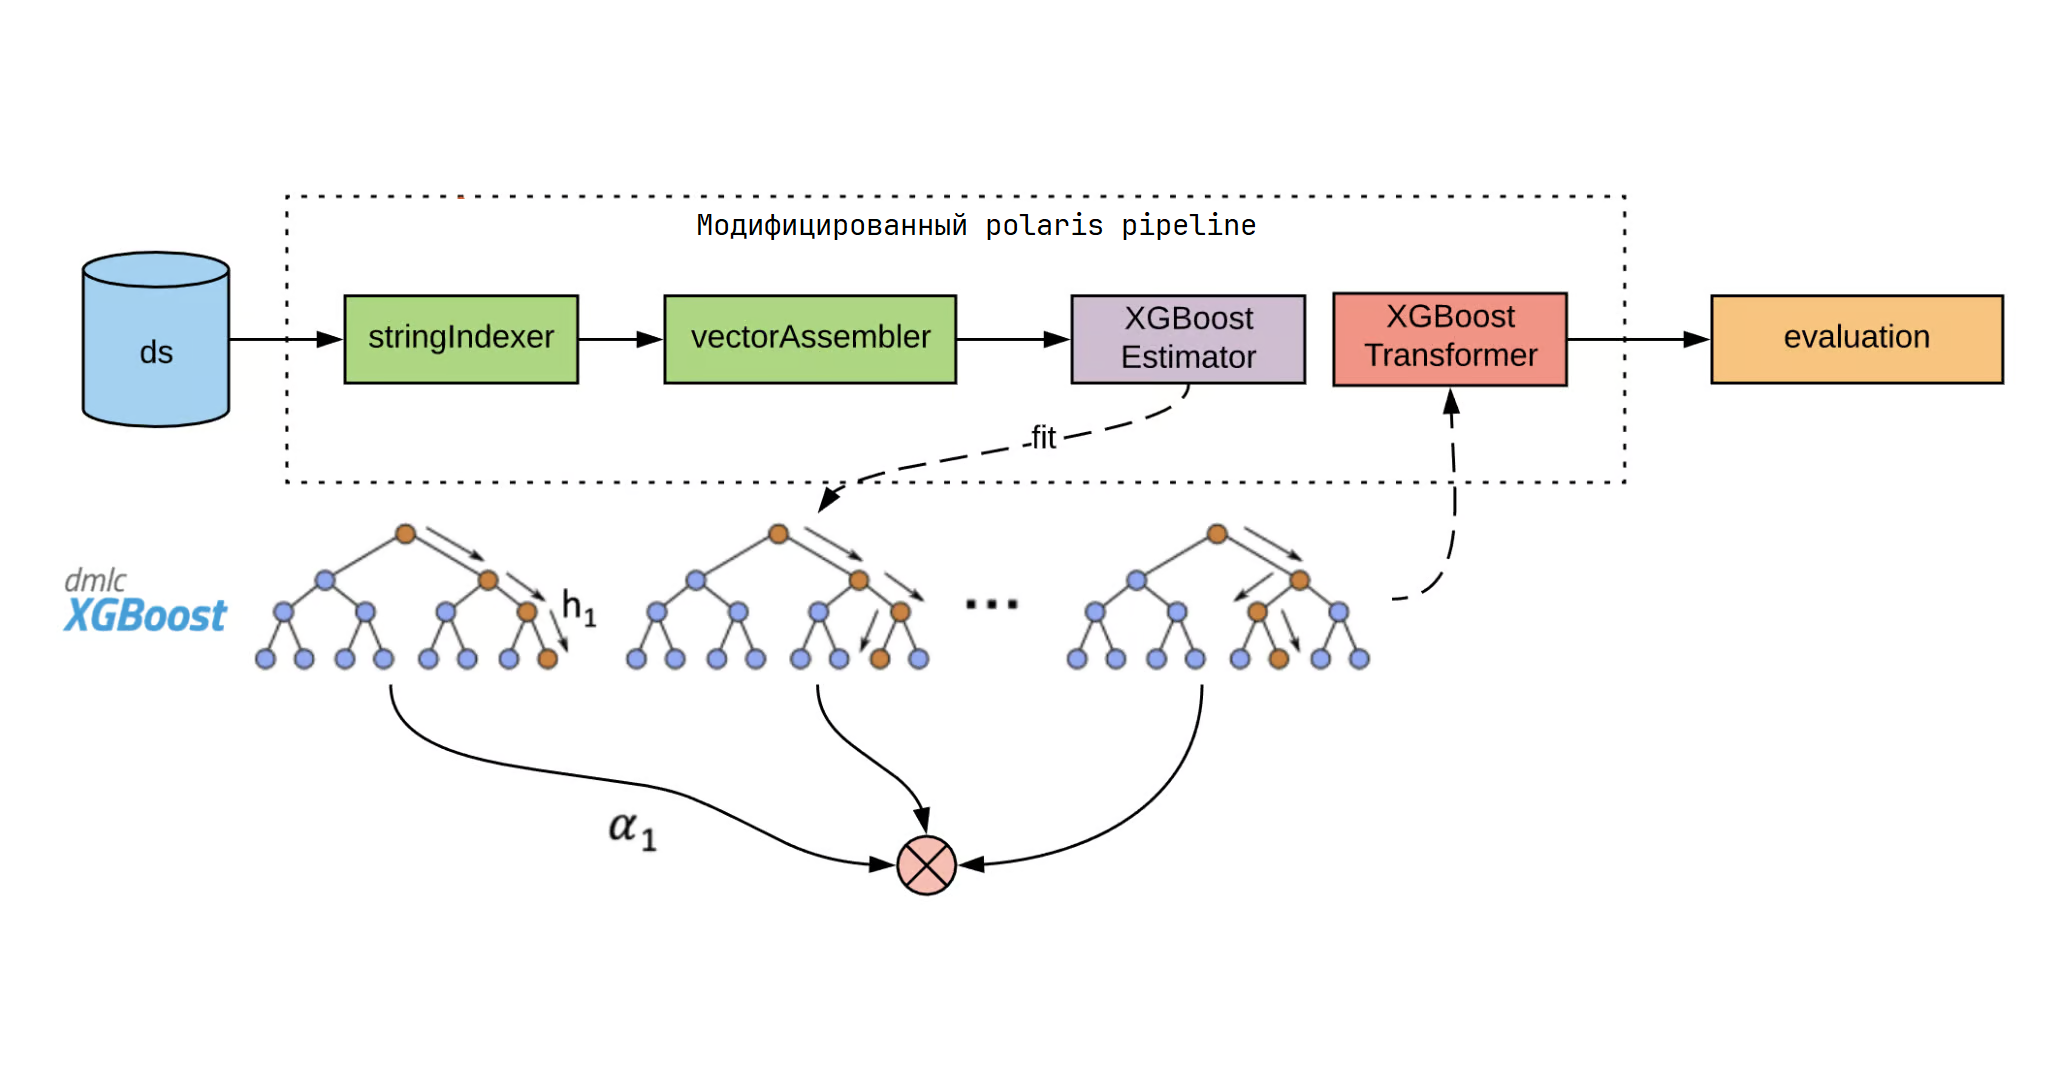
\includegraphics[width=1.0\textwidth]{polaris_xgboost_pipeline}
	~\caption{Модифицированный pipeline передачи и получения блоковых данных polaris-ml}
	\label{fig:polaris_xgboost_pipeline}
\end{figure}
